\documentclass{beamer}
\usepackage{wasysym}

\usepackage[framemethod=tikz]{mdframed}
\usepackage[makeroom]{cancel}
\usepackage{tikz}

\tikzstyle{every picture}+=[remember picture]
\usetikzlibrary{arrows,positioning}
\tikzset{
	%Define standard arrow tip
	>=stealth',
	%Define style for boxes
	punkt/.style={
		rectangle,
		rounded corners,
		draw=black, very thick,
		text width=6.5em,
		minimum height=2em,
		text centered},
	% Define arrow style
	pil/.style={
		->,
		thick,
		shorten <=2pt,
		shorten >=2pt,}
}
\usetikzlibrary{positioning}

\usetheme[sectionpage=none,numbering=counter]{metropolis}
%\setbeamertemplate{footline}[frame number]
\usepackage{graphicx}
\usepackage[utf8]{inputenc}
\usepackage[T1]{fontenc} 
\newcommand{\textoverscript}[1]{$^{\text{#1}}$}
\newcommand{\textunderscript}[1]{$_{\text{#1}}$}
\usepackage{caption}
\captionsetup{justification=raggedright,singlelinecheck=false}
\captionsetup[figure]{labelformat=empty}


\setbeamercovered{transparent}% Dim out "inactive" elements
\setbeamertemplate{caption}{\raggedright\insertcaption\par}
\setlength\abovecaptionskip{-15pt}
\newcommand{\tabitem}{%
  \usebeamertemplate{itemize item}\hspace*{\labelsep}}
\title{He$^+$ Pickup Ion Measurements\\ with Ulysses SWICS}
\subtitle{MNF-phys-1321}
%\subtitle{MNF-phys-1321 -- Methodenkenntnisse und Projektplanung}
\author{Anne Fischer}
\date{\today}
%
%
%
\begin{document}

%%%
\section{Pickup Ions}
\subsection{Basics}
\begin{frame}{Pickup Ions Basics}

\begin{figure}
	\vspace{-1.cm}
	\hfill
	\hspace{3.7cm}
	\hfill
	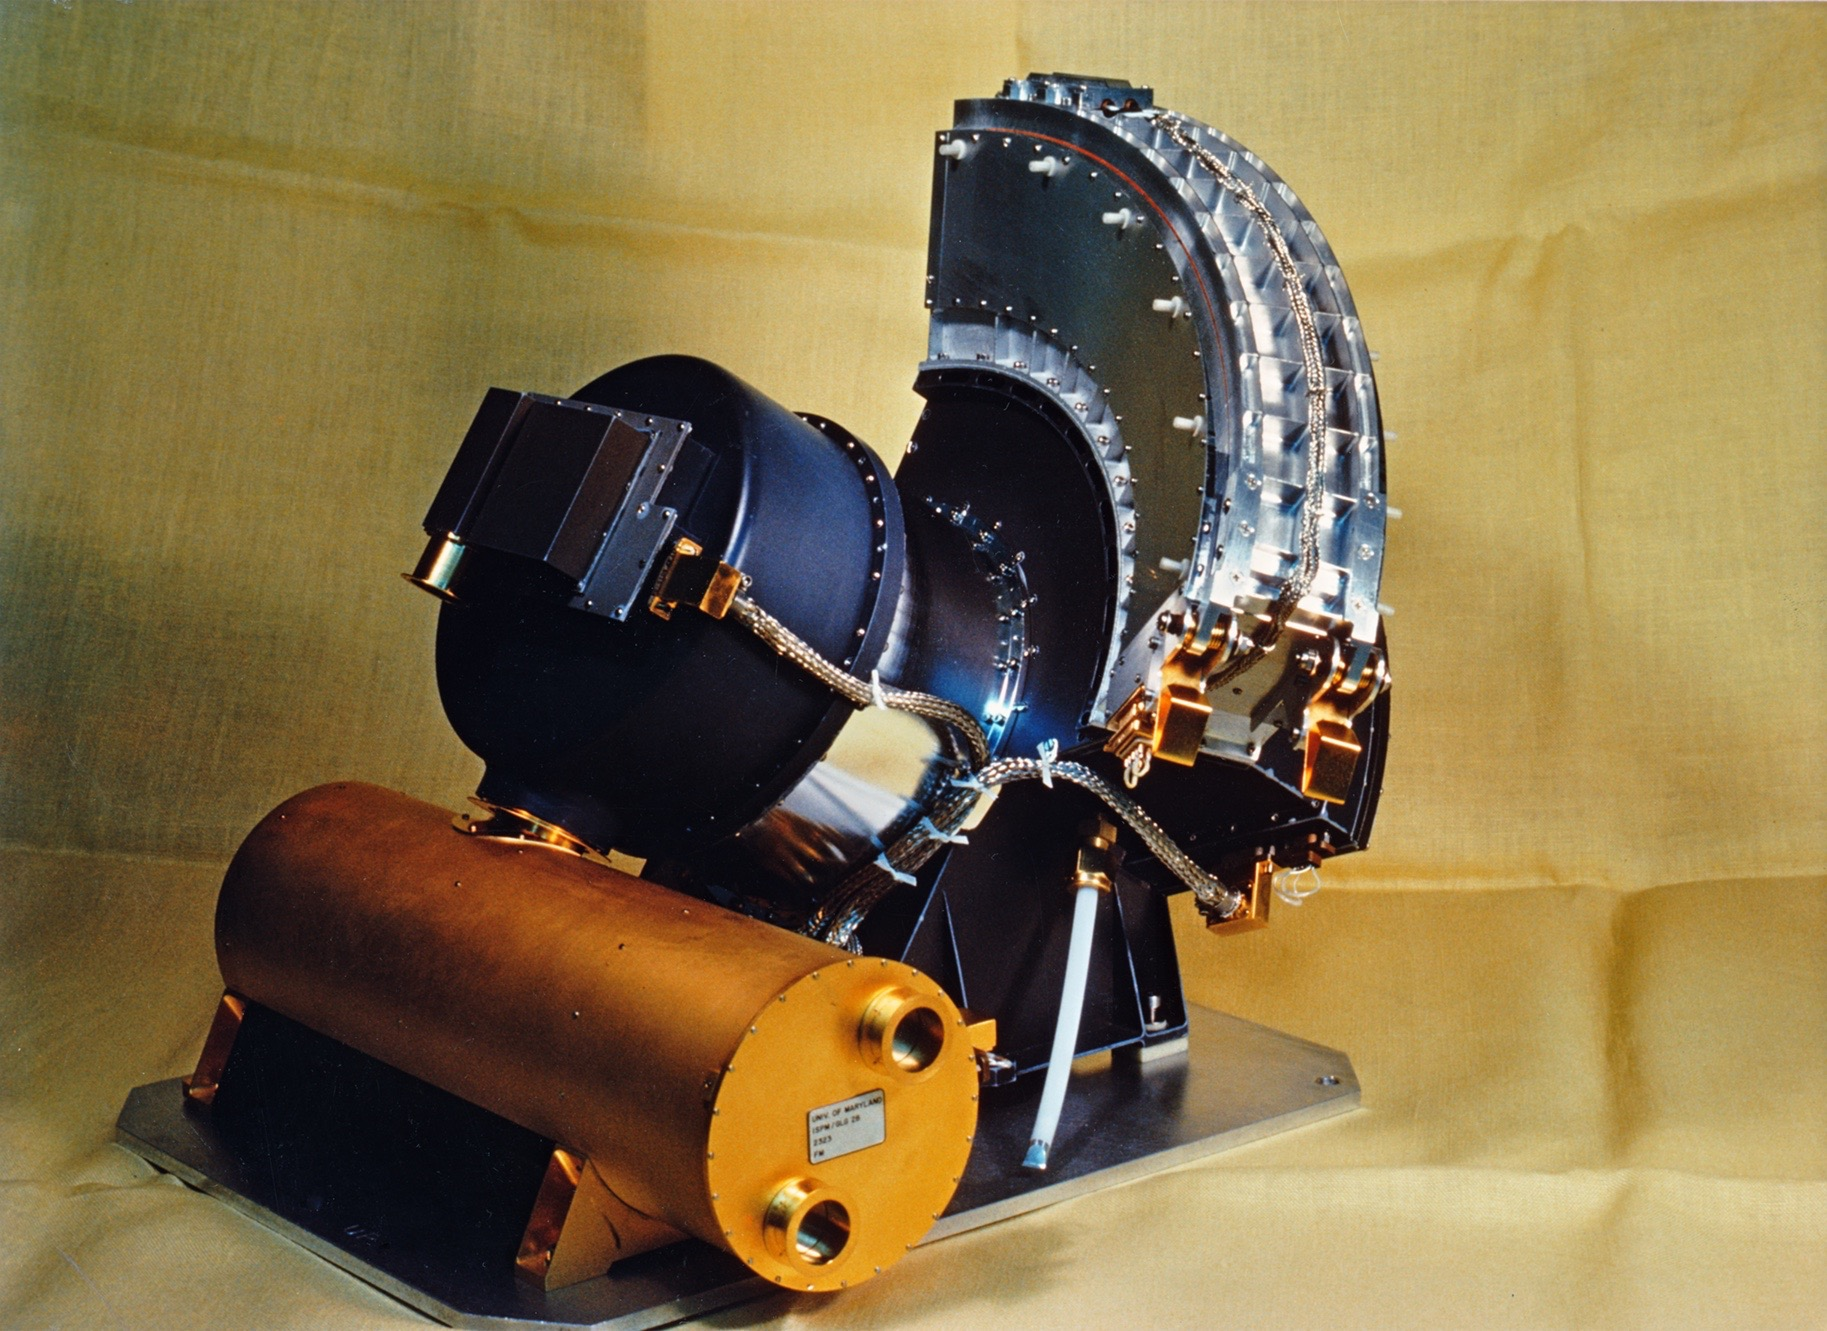
\includegraphics[scale=0.04]{Pics/ULYSSES-SWICS.jpg}
	
	\vfill
								
\end{figure}


	\begin{columns}

	\column{5cm}
	test

	\column{5cm}
	\begin{figure}
		\hspace{2cm}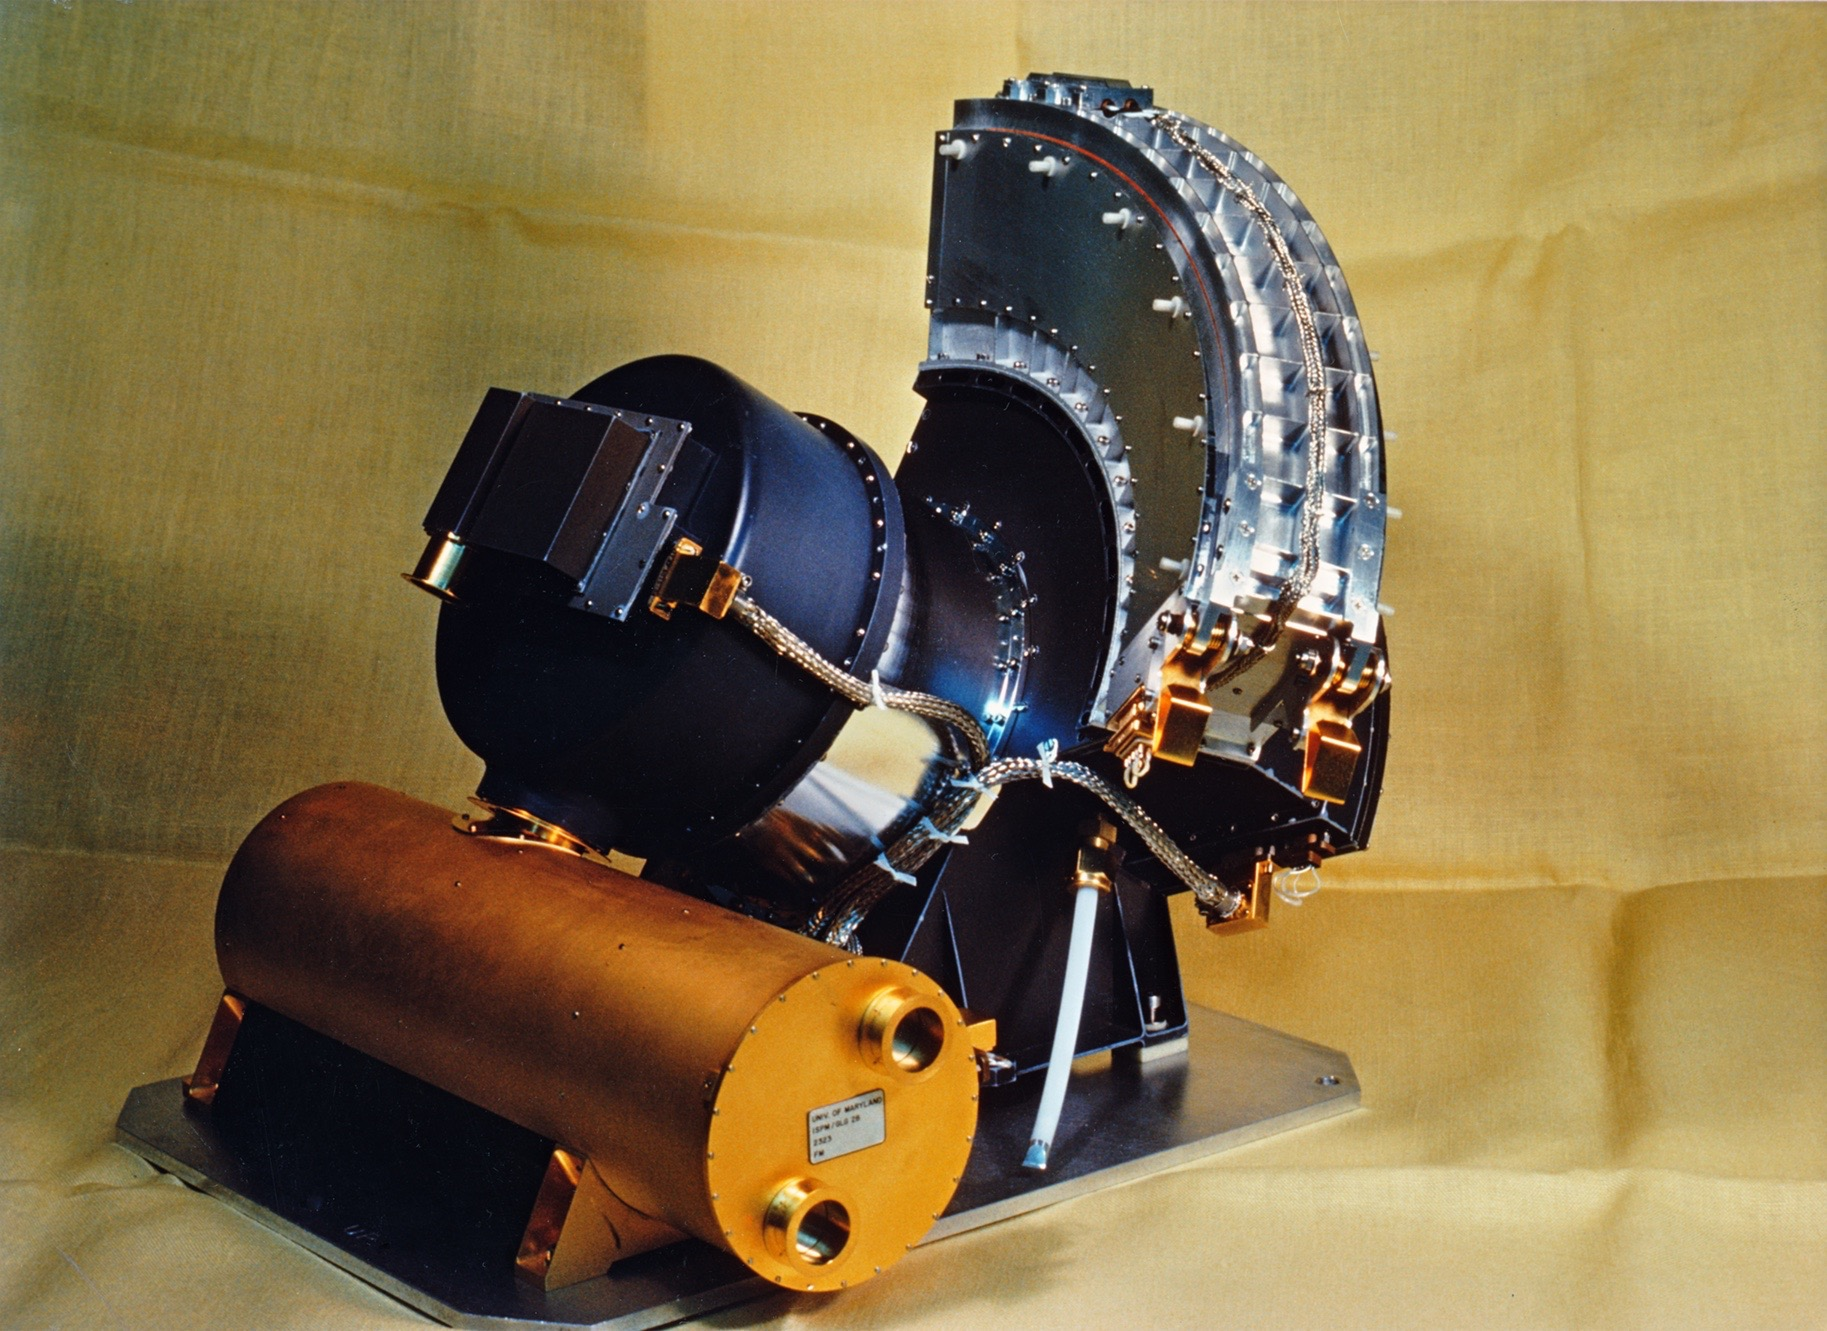
\includegraphics[scale=0.06]{Pics/ULYSSES-SWICS.jpg}
		\vspace{0.1cm}							
		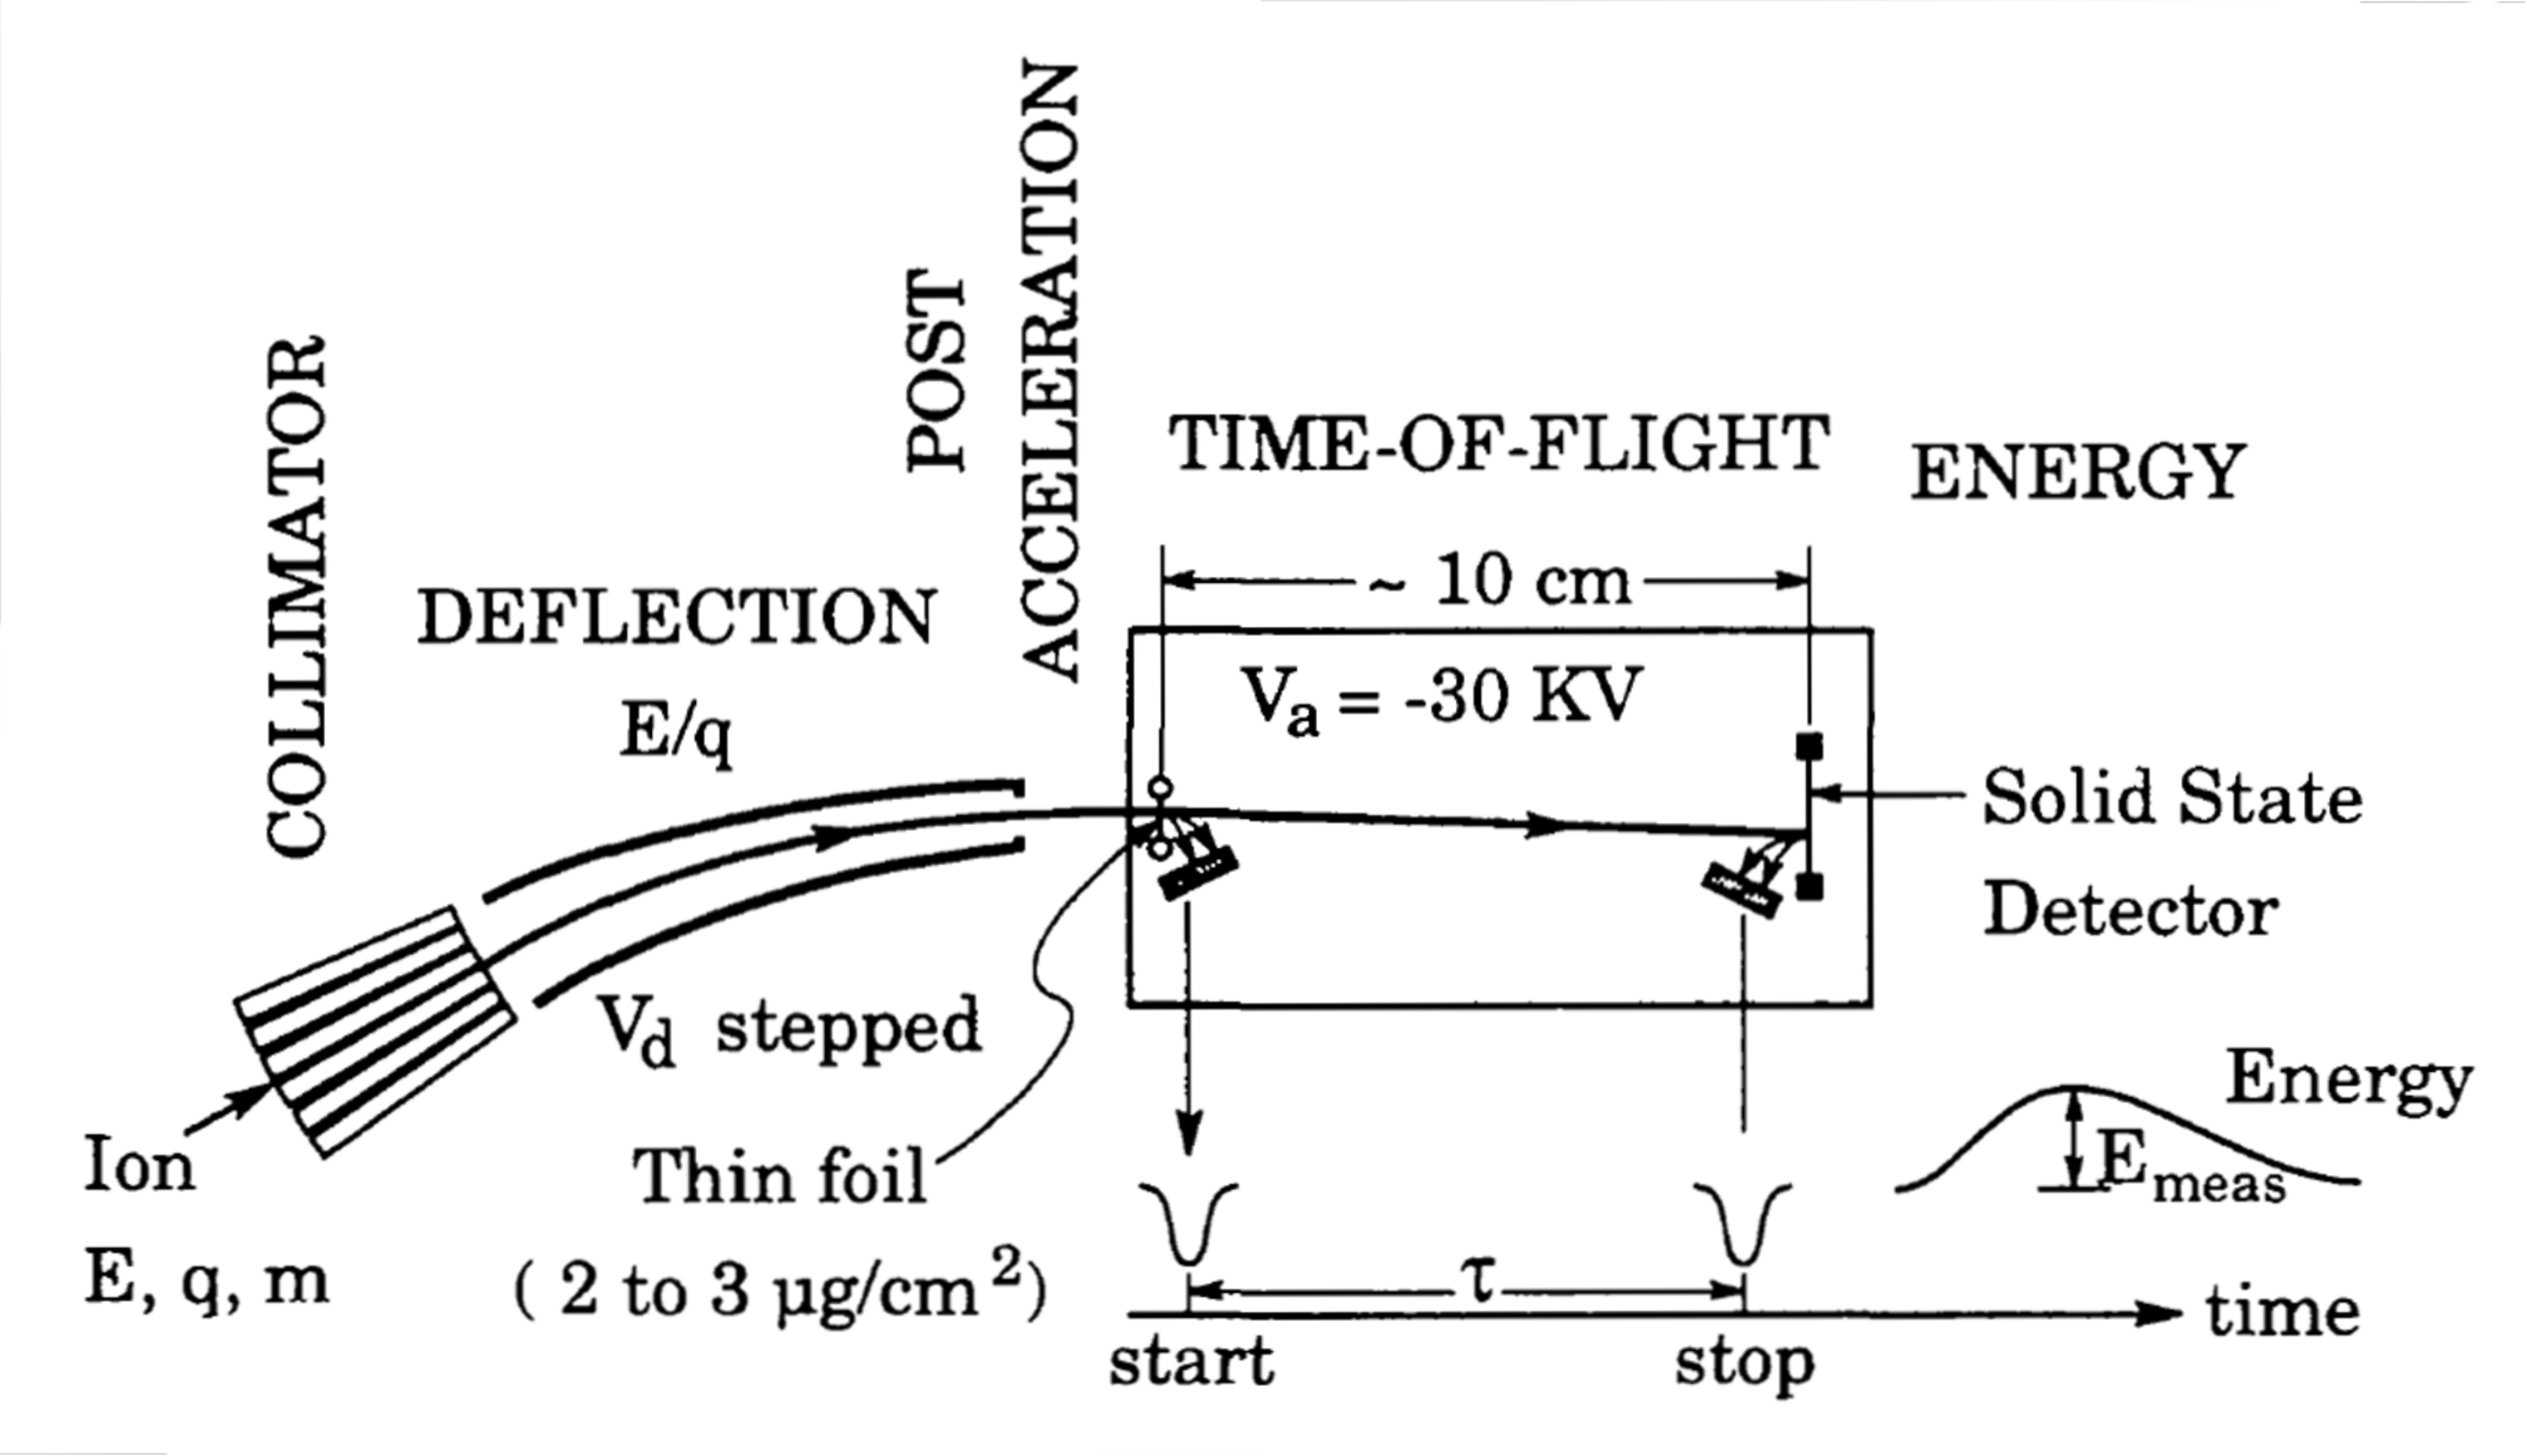
\includegraphics[scale=0.15]{Pics/SWICS_measurement_gerade.pdf}
		\caption{\tiny{\begin{center}
		\textit{Gloeckler, Geiss et al., 1992}\end{center}}}
	\end{figure}
		
	\end{columns}
\end{frame}
%
%
%
\end{document}